%\documentclass[a4paper,12pt]{report}
\documentclass[oneside,12pt]{uafthesis}


%allows for hyperlink
\usepackage{hyperref}
%re-define how \autoref (found in hyperref package) prints a chapter reference
%Default is "chapter", but I want "Chapter" instead
\renewcommand*{\chapterautorefname}{Chapter}
%\usepackage{url}

%allows for degree symbol, among other things presumably
\usepackage{textcomp}

%draws bounding boxes around the major page elements. For troubleshooting
%\usepackage[showframe]{geometry}


%allows multiple rows in a single column withing a table
\usepackage{multirow}

\usepackage{amsmath, amssymb, amsfonts} % Thanks, AMS!
%\usepackage{fixltx2e} % Allows \(\) in captions, amongst other things.
%\usepackage{ppl} % The Paladino font (tough to find?)
%\usepackage{pxfonts} % Paladino-like fonts
\usepackage{graphicx, float} % Graphics stuff
\usepackage[space]{grffile}
\usepackage{verbatim} % Mostly for the comment environment.
%\usepackage{chapterbib} % This is an option for those bundling papers.
%\usepackage[square]{natbib}
%\usepackage{tocbibind} % This fixes the "bibliography in ToC" problem.
                        % Use with chapterbib.
\usepackage{booktabs}                       
\usepackage{cancel}
%\usepackage{caption}
\usepackage{cleveref}
\usepackage{colortbl}
\usepackage{csquotes}
\usepackage{helvet}
\usepackage{mathpazo}
\usepackage{listings}
\usepackage{pgfplots}
\usepackage{xcolor}
%\usepackage{translator}
%\usepackage{beamer}

%For using units in equation mode 
\usepackage{siunitx}
\DeclareSIUnit\rpm{rpm}
\DeclareSIUnit\voltamp{VA}
\DeclareSIUnit\voltampreactive{VAR}

%Allows for drawing circuit diagrams
%\usepackage[siunitx]{circuitikz}
\usepackage{circuitikz}

%Not sure exactly why this line is needed but I got a warning that said: running in backwards compatibility mode (unsuitable tick labels; missing features). Consider writing \pgfplotsset{compat=1.16} into your preamble.
\pgfplotsset{compat=1.16}

%certain default hyphenations aren't what I want
\hyphenation{geo-ther-m-al}

%Various title/signature page info
\author{Nathan Green}
\title{Prime Power Generation and Distribution in Microgrids with Geothermal Organic Rankine Cycle Turbine and Self Excited Induction Generator}

\degreeyear{2018}
\degreemonth{}
\degree{Master of Science}
%\degreesubject{Electrical Engineering}
\department{Electrical \& Computer Engineering}
\numberofmembers{3} % Make sure this is right! The grad school hates empty
                    % signature lines.
\committeechair{Richard Wies}
\committeememberfirst{Daisy Huang}
\committeemembersecond{Mari Shirazi}
\departmentchair{Charlie Mayer}
\collegedean{Douglas Goering}
\graddean{Michael Castellini}

\committeewidth{4in}
\approvedwidth{4in}
\comitteespace{\hfill}
\approvedspace{\hfill}

\prevdegrees{B.S.}
\college{College of Engineering \& Mines}

\begin{document}

%\makesig
\maketitle
\begin{abstract}

Diesel electric generation is heavily used in remote permanently islanded microgrids, even in areas where alternative resources are readily available. The cost of diesel fuel for these generators is high in part because of the difficulty in transportation. Additionally, as the cost of fuel increases, so too does the cost of transportation, hitting these remote communities harder. This thesis will show that local resources such as geothermal hot springs can provide primary for these remote microgrids, even at relatively low temperatures below the boiling point of water. The geothermal heat will be processed with organic Rankine cycle in combination with a self excited induction generator. A steady-state energy balance model will be devoloped using MATLAB Simulink. The model will be used to simulate greenfield and brownfield geothermal microgrids at Pilgrim Hot Springs, Alaska and Bergssta$\eth$ir, Iceland respectively to demonstrate viability of this microgrid design. 

%A stability analysis will be conducted using the long and short term simulation models which evaluate system voltage and frequency under different conversion topologies. A cost analysis will also be conducted to compare the economic viability of operating the different systems in remote communities. It is expected the system with greatest stability will not be the most cost-effective, but that there is a system which provides stable power within reasonable tolerances at optimal cost.

\end{abstract}


%Table of Contents and such
\tableofcontents
\listoffigures
\listoftables
%\listofothermaterials
%\listofappendices

%Each chapter is included
\chapter{Introduction}
\label{ch:intro}

\section{Problem Statement}
The state of Alaska currently has dozens of communities which are electrically isolated from the rest of the state. They effectively act as remote permanently islanded microgrids. These communities typically use diesel generators to provide most of their electrical power. Power sources such as coal or natural gas are less expensive in larger grids, but these microgrids are too small to take advantage of such economies of scale. This makes it expensive to operate relative to the size of the communities. Furthermore, the remoteness of these communities significantly increases the cost to import fuel.

The goal of this thesis is to determine an affordable method to incorporate renewable energy into microgrids without compromising stability and reliability. One method of reducing operating costs is to offset diesel fuel through the use of locally available renewable energy resources.\footnote{Sometimes called renewables, these sources of energy either will not be depleted or can be replenished in a reasonably short period of time. They include wind, solar, geothermal heat, biomass, and water flow.} Unfortunately powering a microgrid with a significant portion of intermittent renewable resources can negatively impact grid stability unless appropriate infrastructure is included. 

This thesis will seek to accomplish its goal by simulating the operation of a permanently islanded microgrid containing geothermal organic Rankine Cycle (ORC) power generation for two types of site applications. In both cases the geothermal power will be converted from AC to DC then back to AC in to be distributed to the loads.
\begin{itemize}
\item One greenfield site will be examined with no existing permanent electrical infrastructure.
\item One brownfield site will be examined where there is an existing grid connection but experiences regular outages.
\end{itemize}
\nomenclature[B]{ORC}{Organic Rankine cycle}

The greenfield area selected for this study, Pilgrim Hot Springs, lies about 60 miles north of Nome in western Alaska. Since the 1970s there has been interest in developing the hot springs in order to generate electricity.  Several exploratory wells have been drilled and indicate potential for low temperature geothermal electrical generation \cite{Holdmann2013}. \autoref{fig:pilgrimFLIR} shows a geothermal runoff stream and how much warmer the water is compared to the banks. The area is currently undeveloped,\footnote{There are historic ruins of an old church and orphanage from the early 1900s, but those buildings are uninhabitable.} therefore, this remote microgrid will be designed from scratch. The land owners, Unataaq LLC, have expressed interest in developing the resource as a tourist attraction, for agriculture, as well as for electrical production. They are currently working with the Alaska Center for Energy and Power (ACEP), a research group at the University of Alaska Fairbanks, to fulfill these goals. 
\begin{figure}[h]
	\centering
	
	\includegraphics[width=\textwidth]{figures/PilgrimFLIR.png} 

	\caption{A FLIR image of a Pilgrim hot springs geothermal runoff stream overlayed onto a photo.}
	\label{fig:pilgrimFLIR}


\end{figure}
\nomenclature[B]{ACEP}{Alaska Center for Energy and Power}

The greenfield system would be similar to the organic Rankine cycle generator used in Chena Hot Springs. Though near Fairbanks, Alaska, these hot springs are not connected to the larger grid, and primarily use diesel generators to produce electric power. In an effort to reduce fuel usage, the owner worked with United Technologies and Carrier Refrigeration to install two 200 kW ORC generators to supplement the diesel generation. At the time of construction, the system found at Chena Hot Springs made use of the lowest temperature geothermal resource for operating ORCs \cite{Holdmann2007}. In addition to the ORCs, Chena uses the geothermal hot water to heat cabins and greenhouses, as well as for sitting pools. 

Iceland has extensive experience utilizing their geothermal resources, but so far only high temperature areas are used for electricity production, while low temperature sites are used for district heating. One such system, and the brownfield case study, heats the community of Bergsta$\eth$ir, Iceland, a rural area in the northern part of the island. \autoref{fig:bergstadir_effluent} shows the discharge pipe and steaming effluent of the system. The pumps used to circulate the water are electrically driven by two \SI{15}{\kilo\watt} motors, but the electrical grid in rural Iceland is less reliable than the heating loop needs to be. Currently the community uses diesel generators to power the pumps during the power outages, but they are interested in alternatives.
\begin{figure}[h]
	\centering

	\includegraphics[width=\textwidth]{figures/BergstadirEffluent.jpg} 

	\caption{District heating effluent at Bergssta$\eth$ir, Iceland. Credit: George Roe.}
	\label{fig:bergstadir_effluent}

\end{figure}

\autoref{fig:abridged_flow_diagram_label} shows a simplified flow diagram of the model using an ORC as the power source. The components include an ORC system as a source, a load, and an inverter to link the source output to the load. In the figure, the blue lines represent electrical connections, while green represents the flow of data and component parameters. The ORC block is composed of evaporating and condensing heat exchangers, an isentropic pump, an isentropic expander, and self-excited induction generator. 
\begin{figure}[ht]
	\centering
	\caption{A simplified diagram of power and data flows of the model. Blue lines represent electrical power connections and flows similar to a one-line diagram. Green boxes data flow from one part of the model to another.}
	\label{fig:abridged_flow_diagram}
	
	%\includegraphics[width=\textwidth]{figures/Abridged Pilgrim Model Flow diagram - AC bus.pdf} 
	\includegraphics[width=\textwidth]{figures/SimpleFlowDiagram.pdf}

\end{figure}

\section{Microgrid Description}
Microgrids are electrical systems composed of sources and loads within a well defined electrical boundary. Many microgrids are connected to a larger grid, but with the ability to become separated, or islanded, while still maintaining some or all of the loads. Others need to remain connected but still maintain a boundary. Some form of energy storage is often used for systems operating independently from the larger grid. This section will describe the key components and characteristics of a microgrid with emphasis on relevance to Alaska.

Approximately 70\% of the population of Alaska is connected to a single grid called the Railbelt \cite{railbelt}. The Railbelt stretches over 600 miles from Homer on the Kenai Peninsula to the greater Fairbanks area in the interior and includes most communities on the road system. The remaining communities and villages can be considered permanently islanded microgrids. Each has loads that need power, some power source, and some system of storing the energy or fuel.

A microgrid can operate using alternating current (AC), direct current (DC), or a hybridization of the two. The choice of whether to use AC\footnote{Unless otherwise noted, AC will refer to three phases separated by a phase angle of 120\textdegree{} rather than a single phase.} or DC depends on the demand of the loads, the available power sources and conversion devices, as well as the existing electrical infrastructure. The decision between AC and DC goes as far back as 1880s when George Westinghouse and Thomas Edison were competing to supply America with electrical power. Ultimately Westinghouse and AC came out on top in part due to its relative ease of transforming to high voltage and low current which transmits more efficiently. Furthermore, electric machinery that uses AC to generate rotating magnetic fields operates more efficiently than machines which use DC power and commutators. Like most of the world, Alaska uses AC networks and converts to DC as necessary at the device level.
\nomenclature[B]{AC}{Alternating current}
\nomenclature[B]{DC}{Direct current}

While AC is still the standard for most power distribution and transmission, DC applications are seeing increased attention. DC interties are already used to connect large areas of the national power grid to act as a buffer for frequency and voltage variations between each part of the system. DC microgrids also have the potential to improve stability with distributed, intermittent, and highly variable renewable generation, although much work is still needed. Integration of AC and DC infrastructure remains challenging for adaption into existing systems, though low-cost solid-state power electronic converters increase the viability of greenfield DC microgrids.
%More recently, however, computers and other electronic devices which use DC have become much more prolific, which has led to a renewed call for DC systems. 

\subsection{Sources}
Microgrid power is typically generated by distributed energy resources (DER). This can include renewable resources such as solar photovoltaics, wind turbine generators, hydrokinetics, biomass, and geothermal-based generators. Some non-renewable DERs include diesel generators and natural gas micro-turbines. 
%Most power sources generate AC power. Current is induced by rotating coils withing a magnetic field
\nomenclature[B]{DER}{Distributed energy resource}

Diesel generators use the combustion of diesel fuel to spin an alternator producing AC power. These generators are prolific in rural Alaska generally being used as the prime mover to regulate grid frequency and voltage. The communities  generally purchase the fuel in bulk once or twice each year because of their remote locations. The fuel is then stored in tank farms.
%These generators are composed of an engine, alternator, fuel system, excitation system, governor, cooling system, exhaust system, and turbocharger.
Due to the widespread use of diesel generators in Alaska, significant energy cost savings can be generated by reducing fuel consumption through efficiency improvements and use of renewable energy sources. 

This thesis is focused on using geothermal generators, in particular, as a prime renewable energy source to displace the fuel consumption of diesel generation. Geothermal generators are heat engines, and operate similarly to traditional coal and nuclear plants. Heat causes a working fluid to thermally expand and change phases thus spinning a turbine to produce AC power. The primary difference is that geothermal systems get heat from the Earth as opposed to combustion or nuclear reactions. Geothermal generators can be divided into high heat and low heat categories. High heat geothermal systems work with temperatures well above the boiling point of water which means water can be used as the working fluid. Low heat systems operate at temperatures near or below the boiling point of water therefore a refrigerant must be used as an alternative working fluid. 
%talk about chena hotspings as an example of existing geothermal in AK

%Wind turbine generators produce what is known as wild AC, where frequency and voltage are unregulated and can vary with wind speed. Modern wind turbines have built-in methods of ensuring the generated power is usable by the grid.
%\begin{verbatim} 
% address gearboxes  
% various wind turbine conversion topologies perhaps
% talk about wind resources of western alaska
%\end{verbatim}

%Solar photovoltaic (PV) panels generate DC power. Panels are made up of a string of cells of a semiconductor material. The most commonly used material is Silicon, but Gallium Arsenide (GaAr), Cadmium Telluride (CdTe), and Copper Indium Gallium Selenide (CIGS) can be used in certain applications as well. Regardless of the material, all PV panels operate by absorbing sunlight and exciting electrons to higher energy orbital. Some fraction of the excited electrons become free and capable of generating a current. PV systems in Alaska face certain challenges due to the long dark winters, however there are also several beneficial characteristics. Solar PV cell operate more efficiently in colder temperatures and reflection due to high albedo of snow can increase the light incident on appropriately positioned panels. During the months of March and April, twelve or more hours of sunlight are available, but temperatures remain relatively cool and the ground remains covered in snow. For those reasons solar PV can be especially competitive in the Alaskan spring.

\subsection{Loads}
Well designed microgrids are configured around expected loads. Loads can require active as well as reactive power. Reactive power cannot do any net work, but is generally used to maintain magnetic or electric fields in inductive loads. Any work done by the field, such as a magnetic field spinning a rotor, is due to active power. Active power, also called real power, is associated with resistive loads. While resistive loads consume active power and inductive loads consume reactive power, capacitive loads generate reactive power and are often used to reduce the reactive power supplied by the sources. 

Regardless of the type of load, there must always be a power balance among sources, loads, storage, and losses. If the total load increases to a high level, either additional sources must be brought online or other loads must be shed. It costs money to bring more sources online, particularly fuel based sources, therefore, it is better to decrease the load if possible. Certain flexible loads can be designated as dispatchable. They require a certain amount of energy over a period of time but not continuously or on demand. These loads can be shut off automatically or forced to remain off during periods of high energy use. Additionally, if the power generated by intermittent renewable resources exceeds the power consumed by normal loads, dispatchable loads can be activated sooner than they otherwise would be. This can potentially maximize fuel displaced by the renewable resources. However, the dispatchable loads require additional infrastructure and controls in order to communicate with other grid components to know when to turn on and off.

\subsection{Storage}
Energy storage is beneficial to microgrid operation because it allows generation to be spread over time. Energy Storage Systems (ESS) can include batteries, flywheels, super-capacitors, pumped hydro, and more. These devices have different storage duration and discharge times making various storage technologies advantageous in different situations \cite{Schoenung2003}. The discharge of bulk energy storage over the course of many hours allows for load leveling and provides spinning reserve for the grid.\footnote{Spinning reserve is extra operating capacity capable of responding to sudden load increases at will.} Load peak shaving typically involves a discharge time from minutes to several hours. Energy storage discharge over seconds and sub-seconds is generally done to improve power quality.
\nomenclature[B]{ESS}{Energy storage system}

%Bulk diesel fuel tanks can provide an alternative method of energy storage.

\subsection{Conversion}
Electronic conversion devices take a form of electrical power (AC or DC) and convert it into a different form. Power conversion devices typically use switching components such as diodes or transistors to control the output voltage and current waveforms.\footnote{The major exceptions are transformers.} Inductors and capacitors provide filtering as well as ensure continuous levels of the voltage and current. Inverters convert DC power into sinusoidal AC power. Rectifiers convert AC to DC. DC-DC converters can step up or down the voltage level of a DC power source. Transformers can step up or down the voltage level of an AC source by magnetic induction while maintaining frequency. Variable frequency drives (VFD)\footnote{Sometimes called Variable Speed Drives (VSD)} modify the frequency of an AC source by rectifying the AC source and then inverting that output back to AC at the desired frequency. 
\nomenclature[B]{VFD}{Variable frequency drive}
\nomenclature[B]{VSD}{Variable speed drive}
%address high frequency transformers: isolation + additional voltage step up/down
%maybe in conversion chapter



%\paragraph{}
%More advanced methods and architectures of power conversion will be addressed further in \autoref{ch:conv}.

\subsection{Control}
A microgrid control system ties all the other components together. Control systems monitor and maintain the voltage and frequency of the grid while ensuring sufficient active and reactive power is supplied to the loads. The control schemes of power sources and converters can generally be divided into several categories: grid forming, grid following, grid supporting, and grid parallel \cite{Ortjohann2012, Engler, Strauss2003}. 

Grid forming units set the frequency and voltage levels of the microgrid. Grid following units control the power\footnote{Both active power and reactive power.} supplied to the grid based on external reference values from the loads. As loads demand more power, a grid following unit will supply more power within its capabilities. Grid supporting units provide power based on voltage and frequency regulation. They assist the grid forming unit with maintaining the voltage and frequency while also supplying power. Grid parallel units also supply power to the grid, but it is based on reference values of a source. These units typically incorporate a maximum power point tracking (MPPT) algorithm in order to produce as much power as is available. They are used with intermittent sources such as wind turbines and solar PV arrays. 
\nomenclature[B]{MPPT}{Maximum power point tracking}

Control over DER and electronic conversion devices can also be categorized by whether or not communication is used. Typically communication among converters can yield more precise power sharing and set points, but the necessary communication lines can introduce additional costs and points of failure \cite{Vandoorn2013}. Furthermore, control strategies that do not require communication are easier to expand and provide redundancy because coordination among controller units is less complex. Methods of communication based control include centralized, distributed, and master\slash slave control. Methods of non-communication based control include droop control as well as frequency based signal injection.

\subsubsection{Communication Based Control}
Centralized control schemes make use of two way communication where a central controller sets the priorities of local DER and load controllers during regular intervals. The priorities are determined from a predefined optimization algorithm and use inputs of power supply and demand from the local controllers, as well as market costs during the previous interval \cite{Katiraei2008}. Distributed control schemes also use a centralized control unit to regulate the set points of the local control units, but simpler communications are used. The central control unit responds more slowly to disturbances than the local controllers, but helps ensure they share power evenly in steady state conditions \cite{Prodanovic2006}. 

In a master\slash slave relationship between different DER units, the master will operate in voltage control mode and the slave units in current control mode. Such a system may or may not include a central controller. Without a central controller, the master sets the current reference for the remaining units \cite{Siri1992}. If there is a central controller then it is the controller, not the master that sets the current references \cite{Chen1995}.

\subsubsection{Non-Communication Based Control}
\label{sec:droop}
The droop control method originated with the relationship between frequency and active power for synchronous machines due to rotating inertia. As load increases the machines in the system will slow and the system frequency will droop or decrease. It has since been adapted into power conversion control schemes as well despite the lack of physical inertia and often referred to as synthetic or virtual inertia. It is mathematically derived from the equation describing active power flow, $P$, through an impedance $ R + jX $ from point 1 to point 2, as seen in \autoref{fig:droop_circuit}.
\begin{figure}[h]
	
\centering


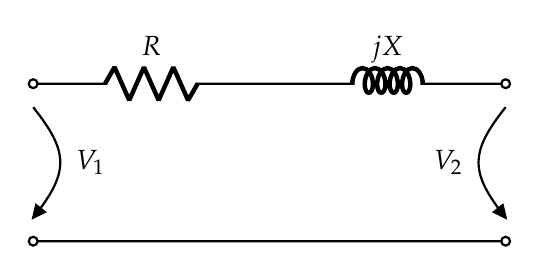
\begin{tikzpicture}
\draw[color=black, thick]
%Input
(0,2) to [open, v^=$V_{1}$, o-o] (0,0){} 
(0,2) to [R, l=$R$] (3,2) to [L, l=$jX$] (6,2) to [open, v=$V_{2}$, o-o] (6,0) -- (0,0){}

;
\end{tikzpicture}
\caption{Circuit diagram of demonstrating power flow from $V_1$ to $V_2$ across impedance $R + jX$.}
\label{fig:droop_circuit}

\end{figure}
\begin{equation}
P = \frac{V_{1}}{R^2 + X^2} \big( R \left( V_{1}-V_{2}\cos{\delta_{12}} \right) +X V_{2} \sin{\delta_{12}} \big)
\end{equation}

Assuming a small phase angle $\delta_{12}$ between the points as well as negligible resistance $R$, the equation can be reduced to 
\begin{equation}
P = \frac{V_1V_2}{X}\delta_{12}
\end{equation}
In practice, the frequency is used rather than the angle because individual units do not know the phase of other units due to the lack of communication. For power and frequency deviation from predefined references the droop equation becomes
\begin{equation}
f = f_{\text{ref}} + K_P\left(P - P_{\text{ref}}\right)
\end{equation}
\nomenclature[V]{$Q$}{Reactive electrical power\nomunit{\si{\voltampreactive}}}
\nomenclature[V]{$f$}{Frequency\nomunit{\si{\hertz}}}
\nomenclature[V]{$V$}{Voltage\nomunit{\si{\volt}}}
where $K_P$ is a negative proportionality constant. 

%\nomenclature[V]{$K_P$}{Negative proportionality constant between change in frequency and change in power in droop control schemes.}


Similarly a droop relationship between reactive power flow and relative voltage levels can be shown:
\begin{equation}
Q = \frac{V_1}{R^2 + X^2} \big( -R V_2 \sin{\delta_{12}} + X \left(V_1 - V_2 \cos{\delta_{12}}\right) \big)
\end{equation}
\begin{equation}
Q = \frac{V_1}{X} \left( V_1 - V_2 \right)
\end{equation}
\begin{equation}
V = V_{\text{ref}} + K_Q \left( Q - Q_{\text{ref}} \right)
\end{equation}
where $K_Q$ is a negative proportionality constant. 

It should be noted, however, that the droop equations are only valid under certain conditions. If the angle\slash frequency deviations are too large then the small angle approximations will break down. Additionally, the relative magnitude of the resistive and reactive impedance components effect system dynamics. If the frequency changes are too large then $X$ can no longer be considered constant. This means the $P$\slash $f$ and $Q$\slash $V$ relationships cannot be approximated as linear. Additionally, the line resistance in most low voltage systems is not so small as to be negligible. In fact in situations where the line reactance is negligible compared to the resistance, linear approximations can be made between active power and voltage as well as reactive power and frequency \cite{YunWeiLi2009}.


%distributed control vs centralized
%droop control vs Master/slave
%Katiraei et al & Vandoorn et al

\section{AC vs DC Microgrids}
AC microgrids and DC microgrids are both technically feasible, but the selection of which is optimal for a given application heavily depends on the types of loads and power sources used. Furthermore, the choice is not necessarily a binary decision. AC\slash DC hybrid systems can provide the benefits of each architecture, but at greater cost. This section will compare and contrast the different architectures.

\subsection{Efficiency}
In each conversion step there is some power loss due to inefficiencies. Sequential conversions can add up to a significant losses. Distributing AC and DC power to their respective loads separately can eliminate many conversion steps but it is unrealistic to completely remove all steps. \autoref{tab:conv_eff} shows that, at rated values, typical losses among different power converters are not symmetric. Transformers are the most efficient, followed by inverters and DC-DC converters. Rectifiers incur the most loss. When operated below rated values all conversion devices experience drops in efficiency.

\begin{table}[]
\centering
\caption{Efficiencies of typical power conversion devices.}
%Keep an eye out for efficiency values more recent the 2006 and 2008
\label{tab:conv_eff}
\begin{tabular}{|ll|l|l|}
\hline
	&				& \multicolumn{1}{l}{From}	&				\\ \cline{3-4} 
	&				& AC				& DC				\\ \hline 
To	& \multicolumn{1}{|l|}{AC}	& 98\% \cite{Starke2008}	& 90\% \cite{Pang2006}	\\ \cline{2-4} 
	& \multicolumn{1}{|l|}{DC}	& 97\% \cite{Starke2008}	& 95\% \cite{Starke2008}	\\ \hline
\end{tabular}
\end{table}
 
% Keep a look out for conversion efficiency more recent than 2006 and 2008

Additionally, distribution power losses are not identical for AC and DC systems. For an AC and DC\footnote{Assuming a DC neutral line introduced.} system, each delivering the same active power and experiencing equal distribution losses, the relationship of RMS current is given as $\frac{I_{AC}}{I_{DC}} = \sqrt{\frac{2}{3}} \approx 0.82$ and a RMS voltage relationship is $\frac{V_{AC}}{2V_{DC}} = \frac{1}{\cos{\theta}} \sqrt{\frac{2}{3}} \approx \frac{0.82}{\cos{\theta}}$ where $\theta$ is the phase angle between $V_{AC}$ and $I_{AC}$ \cite{Starke2008}. Despite the small advantage of DC has over AC in this respect, distribution losses are typically smaller than losses due to conversion.

\subsection{Stability}
Electric machinery and power electronic conversion devices introduce undesired harmonics into AC grids due to non-linear loading effects \cite{Grotzbach1997}. Harmonic distortion can cause power losses as well as reduce voltage and frequency stability. Because harmonics are, by definition, based off of a fundamental frequency the harmonics alone are not an issue in DC segments of a microgrid system. DC systems can experience stability issues caused by non-linear loads such as spikes in current and voltage.

Another important factor in grid stability is how quickly and safely the system can clear an electrical fault. The sinusoidal oscillation of AC systems means there is a periodic zero crossing 60 times each second.\footnote{For regions that operate on 60 Hz.} This means faults can be cleared more quickly in AC systems than in DC systems.  However, AC systems typically experience larger transient spikes during fault events when compared to comparable DC systems \cite{Estes2011}. 

\subsection{Economics}
Most existing electrical infrastructure is built around AC grids rather than DC grids. Furthermore off the shelf electrical appliances generally assume AC power is available and will rectify to DC if needed. These factors indicate the installation of an AC distribution system is more economical. However, AC systems require three lines for each phase, and sometimes a forth neutral line, while DC systems only require two, and sometimes a third neutral line.\footnote{Although work has been done on Single Line Ground Return systems which only require one line.} Although the economic benefit of fewer electrical lines is much more significant to long distance transmission rather than distribution to near by loads.

One benefit of DC microgrids over AC is the necessity to control only voltage level rather than voltage and frequency. A simplified control scheme can reduce the cost combining power sources into a DC bus before distribution avoids the necessity of synchronization \cite{Lotfi2015}.

\section{Thesis Organization}
With the background information on microgrids addressed in \autoref{ch:intro} above, the remainder of the thesis is organized as followed. \autoref{ch:conv} will delve deeper into background of power conversion. This includes the conversion of heat to electricity, with a focus on low-temperature sources, as well electrical power conversion, focusing on the pros and cons of different topologies. 
%\autoref{ch:geothermal} will address necessary background on geothermal power generation. 
\autoref{ch:model} will detail development of the ORC and asynchronous model and its validation. \autoref{ch:analysis} will analyze the simulation results of the greenfield and brownfield scenario.  \autoref{ch:conclusion} will conclude the thesis and describe future work to be conducted on the topic.

\cleardoublepage

\chapter{Energy Conversion}
\label{ch:conv}

Energy and power take many different forms, from the initial sources and to the end results used. Necessarily, methods have been developed to convert the different forms of energy or power from one to another. The first method addressed in this chapter is the conversion of heat to mechanical energy to electrical energy found in heat engines and generators. Next conversion between different forms of electrical power will be addressed.

%This file used to contain the geothermal chapter, now contains thermal/mechanical section of the conversion chapter
\section{Thermal Energy}
Thermal energy, or heat, can originate from many different sources including combustion of a fuel, radioactive decay, or absorption of light from the sun. Heat can be used directly to warm a building, but it is also a critical step in most traditional methods of generating electrical power. 
%\chapter{Geothermal Energy}
%\label{ch:geothermal}

\subsection{Enthalpy}
Enthalpy describes the energy of a system available to be converted to work. It is related to the temperature of the geothermal resource, but also dependent on the pressure and volume. Temperature is usually the primary metric of a geothermal resource, but even a high temperature source is useless without sufficient volume flow. Quantitatively enthalpy is expressed as 
\begin{equation}
H = U + pV
\end{equation}
where $U$ is the internal energy, which is function of temperature, $p$ is the pressure of the system, and $V$ is the volume. Generally it is more convenient to use the change in enthalpy rather than absolute values. After any a system undergoes some thermodynamic process the system will always have some remaining internal energy, pressure, and volume. Therefore a change in enthalpy better describes the energy extracted from (or absorbed by) the system.

Geothermal systems can be classified as high-, medium-, or low-enthalpy\footnote{While the technical definitions differ, the terms enthalpy, heat, and temperature are often used interchangeably when describing geothermal sources.}. Although there is no formal delineation, high-enthalpy sources generally have temperatures greater than about $150$ \textcelsius{} ($302$ \textdegree{}F) and low-enthalpy sources have temperatures lower than $100$ \textcelsius{} ($212$ \textdegree{}F) \cite{Norden2011}. Depending on the amount of extractable energy of the resource, different geothermal processes or cycles should be used.

\subsection{Geothermal Cycles}
%%Describe each of the following but focus on cycles for low enthalpy sources


\subsubsection{Dry Steam}
This high-enthalpy processes extracts hot steam from the earth. The steam is sent directly through a turbine then condensed into liquid water and injected back underground. 

\subsubsection{Flash Steam} 
In the flash steam process high pressure hot is water extracted then allowed to boil becoming steam and low pressure hot water. The steam is sent through a turbine then condensed, recombined with water, and injected back underground.

\subsubsection{Binary Cycle} 
As the name implies, binary cycles involve two loops: a heat source loop and working fluid loop. Heat is collected in the heat source loop and transferred to the working loop through a heat exchanger. The working fluid then undergoes the vaporization process to spin a turbine or screw expander. Binary cycles are technically not limited to low- or medium-enthalpy resources, however high-enthalpy system can be implemented directly with a single loop using the flash or dry steam processes. The most common binary cycle is the Organic Rankine Cycle (ORC) which uses an organic working fluid such as refrigerants. Working fluids are selected for low vaporization temperatures relative to water.

%\subsubsection{(Organic) Rankine Cycle}
%\subsubsection{Kalina Cycle}

\subsection{Synchronous and Asynchronous Generators}
%This section should focus the difference between the two with respect to geothermal sources. I can have a fundemental description of the generators either in this chapter or the intro chapter.

%Direct drives

%\subsection{Pilgrim Hot Springs}
%More thourough description of the resource and potential development plans.

\subsection{ORC Manufacturers and Developers}
\subsubsection{Under Development}
\begin{description}
\item[Air Squared]
\item[Termo2Power]
\item[Climeon]
\item[Calnetix/Access Energy]
\item[Verdicorp] has a range of variable speed expanders. The expander connects to the rotor of a permanent magnet synchronous generator. An IGBT variable frequency drive converts and synchronizes the power with a local grid.
\item[Inifinity Turbine]
\item[Ener-G-Rotors]
\item[Phoenix]
\end{description}
\subsubsection{Commercial Products}
\begin{description}
\item[Electratherm] makes use of a twin screw expander to spin an induction generator.
\item[E-Rationale] uses a single screw expander to rotate an induction generator.
\item[Exergy] %radial outflow turbine
\item[Zuccato] uses a radial inflow turbine directly connected to synchronous permanent magnet generator. Electric power is converted and synchronized to local power grid with IGBT switching.
\item[Enogia] uses a turboexpander. Electric power is rectified then tied into the grid with a grid feed inverter.
\item[Clean Energy Technologies] %uses high speed turbine 
\item[Tri-O-Gen] %uses high speed turbine 
\end{description}
 %used to contain geothermal chapter, now contains thermal section

\section{Electric Conversion}

\subsection{Linear Power Supplies}
%Linear

\subsection{Switched Mode Power Supplies}

\subsection{PWM vs PFM}

\subsection{DC-DC}
recent developments

\subsection{Rectifiers}
recent developments

\subsection{Inverters}
recent developments

%%This file used to contain the geothermal chapter, now contains thermal/mechanical section of the conversion chapter
\section{Thermal Energy}
Thermal energy, or heat, can originate from many different sources including combustion of a fuel, radioactive decay, or absorption of light from the sun. Heat can be used directly to warm a building, but it is also a critical step in most traditional methods of generating electrical power. 
%\chapter{Geothermal Energy}
%\label{ch:geothermal}

\subsection{Enthalpy}
Enthalpy describes the energy of a system available to be converted to work. It is related to the temperature of the geothermal resource, but also dependent on the pressure and volume. Temperature is usually the primary metric of a geothermal resource, but even a high temperature source is useless without sufficient volume flow. Quantitatively enthalpy is expressed as 
\begin{equation}
H = U + pV
\end{equation}
where $U$ is the internal energy, which is function of temperature, $p$ is the pressure of the system, and $V$ is the volume. Generally it is more convenient to use the change in enthalpy rather than absolute values. After any a system undergoes some thermodynamic process the system will always have some remaining internal energy, pressure, and volume. Therefore a change in enthalpy better describes the energy extracted from (or absorbed by) the system.

Geothermal systems can be classified as high-, medium-, or low-enthalpy\footnote{While the technical definitions differ, the terms enthalpy, heat, and temperature are often used interchangeably when describing geothermal sources.}. Although there is no formal delineation, high-enthalpy sources generally have temperatures greater than about $150$ \textcelsius{} ($302$ \textdegree{}F) and low-enthalpy sources have temperatures lower than $100$ \textcelsius{} ($212$ \textdegree{}F) \cite{Norden2011}. Depending on the amount of extractable energy of the resource, different geothermal processes or cycles should be used.

\subsection{Geothermal Cycles}
%%Describe each of the following but focus on cycles for low enthalpy sources


\subsubsection{Dry Steam}
This high-enthalpy processes extracts hot steam from the earth. The steam is sent directly through a turbine then condensed into liquid water and injected back underground. 

\subsubsection{Flash Steam} 
In the flash steam process high pressure hot is water extracted then allowed to boil becoming steam and low pressure hot water. The steam is sent through a turbine then condensed, recombined with water, and injected back underground.

\subsubsection{Binary Cycle} 
As the name implies, binary cycles involve two loops: a heat source loop and working fluid loop. Heat is collected in the heat source loop and transferred to the working loop through a heat exchanger. The working fluid then undergoes the vaporization process to spin a turbine or screw expander. Binary cycles are technically not limited to low- or medium-enthalpy resources, however high-enthalpy system can be implemented directly with a single loop using the flash or dry steam processes. The most common binary cycle is the Organic Rankine Cycle (ORC) which uses an organic working fluid such as refrigerants. Working fluids are selected for low vaporization temperatures relative to water.

%\subsubsection{(Organic) Rankine Cycle}
%\subsubsection{Kalina Cycle}

\subsection{Synchronous and Asynchronous Generators}
%This section should focus the difference between the two with respect to geothermal sources. I can have a fundemental description of the generators either in this chapter or the intro chapter.

%Direct drives

%\subsection{Pilgrim Hot Springs}
%More thourough description of the resource and potential development plans.

\subsection{ORC Manufacturers and Developers}
\subsubsection{Under Development}
\begin{description}
\item[Air Squared]
\item[Termo2Power]
\item[Climeon]
\item[Calnetix/Access Energy]
\item[Verdicorp] has a range of variable speed expanders. The expander connects to the rotor of a permanent magnet synchronous generator. An IGBT variable frequency drive converts and synchronizes the power with a local grid.
\item[Inifinity Turbine]
\item[Ener-G-Rotors]
\item[Phoenix]
\end{description}
\subsubsection{Commercial Products}
\begin{description}
\item[Electratherm] makes use of a twin screw expander to spin an induction generator.
\item[E-Rationale] uses a single screw expander to rotate an induction generator.
\item[Exergy] %radial outflow turbine
\item[Zuccato] uses a radial inflow turbine directly connected to synchronous permanent magnet generator. Electric power is converted and synchronized to local power grid with IGBT switching.
\item[Enogia] uses a turboexpander. Electric power is rectified then tied into the grid with a grid feed inverter.
\item[Clean Energy Technologies] %uses high speed turbine 
\item[Tri-O-Gen] %uses high speed turbine 
\end{description}
	%Electronic conversion and thermal/mechanical conversion chapters combined
\chapter{Model Description}
\label{ch:model}

The model attempts to recreate a microgrid which uses some form of DER as a primary power source along side energy storage in order power the load. \autoref{fig:abridged_flow_diagram} shows a simplified flow diagram of the model using an ORC for the DER. The components include a ORC as a source, a load, and an inverter to link the source two. In the figure, the blue lines represent electrical connections, while green represents the flow of data and component parameters. The ORC block is made up of heat exchangers, an isentropic pump, an isentropic expander, and an induction generator. 
\begin{comment}
The load block \verb|one line description of load|. 
The energy storage block \verb|one line description of energy storage|. 
The inverter block \verb|one line description of inverter|.
\end{comment}
\begin{figure}[ht]
	\centering
	\caption{A simplified diagram of power and data flows of the model. Blue lines represent electrical power connections and flows similar to a one-line diagram. Green boxes data flow from one part of the model to another.}
	\label{fig:abridged_flow_diagram}
	
	%\includegraphics[width=\textwidth]{figures/Abridged Pilgrim Model Flow diagram - AC bus.pdf} 
	\includegraphics[width=\textwidth]{figures/SimpleFlowDiagram.pdf}

\end{figure}

\section{Organic Rankine Cycle Generator}
The ORC generator block links the thermal, mechanical, and electric components of them model. The thermal properties of the fluids were obtained from a Matlab wrapper of the CoolProp library. \cite{Bell2014} Thermal conditions of source, sink, and working fluids are fed into the Rankine Cycle portion of the model, which returns a mechanical power. Electrical conditions, along with the mechanical power, are fed into the generator portion of the model, which returns an electrical output.  

\subsection{Evaporator and Condenser}
The evaporator and the condenser are both represented using a heat exchanger script.  The function takes as inputs parameters about the high and low temperature fluids, specifically the inlet temperatures or enthalpies ($\si{\kelvin}$ or $\si{\joule\per\kilogram}$), mass flow rates ($\si{\kilogram\per\second} $), inlet pressures ($\si{\pascal}$), and fluid names, as well as parameters about the exchanger itself such as the overall heat transfer coefficient ($\si{\watt\per\kelvin\per\meter\squared}$), the heat transfer area ($\si{\meter\squared}$), and the heat exchanger type (e.g. counter or parallel flow). The function output is made up of the heat flow rate ($\si{\watt}$), and the temperatures or enthalpies at the outlets ($\si{\kelvin}$ or $\si{\joule\per\kilogram}$). 

In order to calculate the desired values, the Number of Transfer Units (NTU) method is used. Described in The Fundamentals of Heat and Mass Transfer, \cite{Incropera} this process calculates the output heat flow, $\dot{Q}$, relative to a theoretical maximum heat flow, $\dot{Q}_{max}$. This potential heat flow would be realized using an infinitely long counter flow geometry and is calculated as
\begin{equation}
\dot{Q}_{max} = C_{min}\left(T_{h,i} - T_{c,i}\right)
\end{equation}
where $C_{min}$ is the smaller heat capacity rate of the hot and cool fluids and $T_{h,i}$ and $T_{c,i}$ are the inlet temperatures of hot and cool fluids respectively. The heat capacity rate is the product of mass flow rate, $ \dot{m} $, and the mass specific heat at constant pressure, $ c_p $. 

The heat flow rates of the hot and cool fluids are related by the effectiveness, $\epsilon$, which is defined as 
\begin{equation}
\label{eq:effectiveness_def}
\epsilon \equiv \frac{\dot{Q}}{\dot{Q}_{max}}
\end{equation}

Numerically, the value of $\epsilon$ is a function of the ratio of the fluids' heat capacities, $C_r = \frac{C_{min}}{C_{max}}$, as well as the exchanger's Number of Transfer Units, $NTU = \frac{U \cdot A}{C_{min}}$, where $U$ is the overall heat transfer coefficient and $A$ is the total heat transfer area. Additionally, the direction of fluid flow changes the method of calculation. In parallel flow heat exchangers, the effectiveness is calculated as
\begin{equation}
\epsilon = \frac{1 - \exp\left[-NTU\left(1 + C_r\right)\right]}{1 + C_r}
\end{equation}
while counter flow devices use
\begin{equation}
\epsilon = \frac{1 - \exp\left[-NTU\left(1 - C_r\right)\right]}{1 - C_r\exp\left[-NTU\left(1 - C_r\right)\right]}
\end{equation}

Once the effectiveness and maximum heat transfer rate are determined, equation \ref{eq:effectiveness_def} is used to calculate the actual rate of heat flow, $\dot{Q}$. Finally, the change in temperature for each fluid is calculated based on their respective heat capacity rates at initial conditions and the rate of heat flowing between them. 
If the change in temperature for either fluid would result in vaporization or condensation, then the values must be recalculated because the specific heat is effectively infinite while the fluid is changing states. 

First, the heat flow rate necessary to have the fluid begin changing its state is determined and the fraction of this value relative to initial heat flow rate is calculated. 
The heat transfer area is reduced by this fraction and the function is re-run inputing the state of the two fluids as the one fluid begins to change phase. If enough heat flows between the two fluids such that the one completes the phase change, then the function is run a third time with the heat transfer area modified again. 

Within this script there are certain assumptions made in order to calculate the output values. The function will not return accurate results if both fluids simultaneously undergo a phase change because the ratio of heat capacities, $C_r$, will be undefined. Additionally, Ambient temperature and associated heat flow to the external environment is not accounted for in the script. Finally, it is assumed the pressure drop from inlet to outlet is negligible for both the high and low temperature fluids. 

\subsection{Expander and Pump}
The expander/turbine and pump components are both modeled by a fluid undergoing non-ideal isentropic expansion or compression. For an ideal isentropic process, the fluid will experience some thermodynamic changes while its internal entropy remains constant. 

The function takes as inputs certain properties of the fluid, such as the inlet temperature or enthalpy ($\si{\kelvin}$ or $\si{\joule\per\kilogram}$), both the inlet and outlet pressures ($\si{\pascal}$), and the mass flow rate ($\si{\kilogram\per\second}$). Also needed is the isentropic efficiency, a unitless parameter of the machine which describes lost power due to deviations from the ideal insentropic process. The function returns the power produced or consumed\footnote{Power is produced if the pressure at the inlet is greater than at the outlet, and consumed if inlet pressure is less than that of the outlet.} ($\si{\watt}$) and the temperature or enthalpy ($\si{\kelvin}$ or $\si{\joule\per\kilogram}$) of the fluid at the outlet.

Using the inputs and the Cool Prop library, the Mass Specific Entropy, $S$, of the fluid is determined for the fluid at the inlet. In an ideal process, this value would remain constant, so it is used to determine the ideal enthalpy of the outlet. Next the ideal power transferred is calculated as 
\begin{equation}
\label{eq:power_enthalpy}
P = \dot{m} \left(H_i - H_o\right)
\end{equation}
where $H_i$ and $H_o$ are the inlet and outlet enthalpies respectively.

To obtain the actual transfered power, the isentropic efficiency is applied to the ideal power such that the ideal is necessarily greater than the actual. When the value of $H_i$ is larger than $H_o$, $P$ is positive\footnote{Power is produced.} therefore efficiency is multiplied. When $H_i$ is less than $H_o$, $P$ is negative\footnote{Power is consumed.} and ideal power is divided by efficiency. After actual transferred power is calculated, equation \ref{eq:power_enthalpy} is used to find $H_o$ and the fluid temperature at the outlet.

\subsection{Induction Generator}
The generator block models a Squirrel Cage Induction Generator (SCIG) in order to convert the mechanical power to an electrical form. Two different function blocks were created for two scenarios: regulated and unregulated. The former is simpler to model, but the generator requires another firm source\footnote{Or an electrical storage-inverter combination.} to maintain its frequency and voltage. For the latter scenario, the generator's frequency and voltage are allowed to vary. Its leads are connected directly to a power converter which maintains the frequency and voltage of the remaining microgrid. 

\subsubsection{Regulated SCIG}
This function block takes several electrical and mechanical parameters as inputs such as the line to line voltage ($\si{\volt}$) and electrical frequency ($\si{\hertz}$) at the leads, the mechanical speed at the shaft ($\si{\rpm}$), the number pole pairs in machine's windings, and coefficients of friction due to bearings ($\si{\watt\per\second}$) and windage ($\si{\watt\per\second\squared}$). Also input are the resistive and inductive impedances ($\si{\ohm}$) of the stator, rotor, and core, as well as the capacitive impedance and equivalent series resistance of external excitation capacitor. The function returns the active ($\si{\watt}$) and reactive ($\si{\voltampreactive}$) power outputs and losses.

\begin{figure}[h]
	
\centering

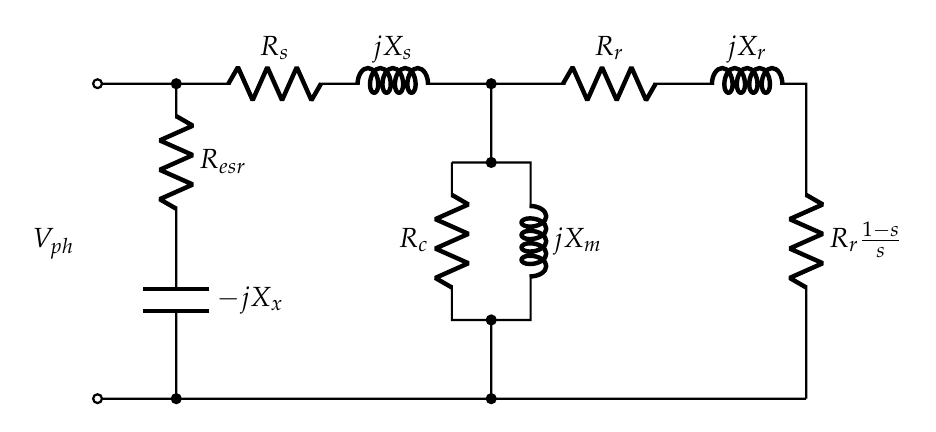
\begin{tikzpicture}[american voltages]
\draw[color=black, thick]
%Input
(0,0) to [open, l=$V_{ph}$, o-o] (0,4){}

%low
(0,0) -- (9,0){}

%stator
(0,4) -- (1.5,4) to [R, l=$R_{s}$] (3,4) to [L, l = $j X_{s}$] (4.5,4){}

%rotor
(4.5,4) -- (5.5,4) to [R, l=$R_{r}$] (7.5,4) to [L, l = $j X_{r}$] (9,4) to [R, l=$R_{r}\frac{1-s}{s}$] (9,0){}

%core
(5,4) to [short, *-*] (5,3){}
(4.5,3) -- (5.5,3) to [L, l = $j X_{m}$] (5.5,1) -- (4.5,1) to [R, l=$R_{c}$] (4.5,3){}
(5,1) to [short, *-*] (5,0){}

%external excitaion capacitor
(1,4) to [R, l=$R_{esr}$, *-] (1,2) to [C, l=$-j X_x$] (1,0.5) to [short, -*] (1,0){}


;
\end{tikzpicture}

\caption{Single phase diagram of a three phase squirrel cage induction machine. $V_{ph}$ and $s$ are the phase voltage and slip of the generator. }
\label{fig:SCIG__circuit_diagram}

\end{figure}
A single phase circuit diagram of the generator which includes these components can be seen in \autoref{fig:SCIG__circuit_diagram}. $R_s$ and $X_s$ represent the resistive and inductive impedances of the stator. $R_r$ and $X_r$ represent the resistive and inductive impedances of the rotor as referred to the stator. $R_c$ and $X_m$ represent the resistive and inductive impedances due to the magnetization of the core. $R_{esr}$ and $X_x$ represent the equivalent series resistance and capacitive impedances of the external excitation capacitor.

To calculate these outputs, first the magnitude of the phase voltage is determined from the line to line voltage, $V_{ll}$, as $ \left|V_{ph}\right| = \frac{\left|V_{ll}\right|}{\sqrt{3}} $ assuming $ \angle V_{ph} = 0\deg $. Next the synchronous mechanical speed is determined by $ n_{synch} = \frac{120f}{2\text{poles}} $ and is used, along with the mechanical speed, $n_{mech}$ to calculate the slip of the machine as $ s = \frac{n_{synch} - n_{mech}}{n_{synch}} $.

The impedances of the stator, rotor, core impedances, the Th\'evenin combination of those three branches, the external excitation branch, and the Th\'evenin combination of all branches are calculated as
\begin{equation*}
Z_s = R_s + jX_s
\end{equation*}
\begin{equation*}
Z_r = R_r\frac{1-s}{s} + R_r + jX_r
\end{equation*}
\begin{equation*}
Z_{core} = R_c \parallel jX_m
\end{equation*}
\begin{equation*}
Z_{machine} = R_s + \left(Z_{core} \parallel Z_r\right)
\end{equation*}
\begin{equation*}
Z_{excite} = R_{esr} - jX_x
\end{equation*}
\begin{equation*}
Z_{total} = Z_{excite} \parallel Z_{machine}
\end{equation*}

Once all the relevant impedances are determined, the currents flowing through the branches are calculated along with the internal voltage at the stator-rotor-core junction. These values are used to determine internal power losses. The mechanical losses due to the bearings and windage are calculated by multiplying the appropriate coefficient of friction by the mechanical angular frequency  and the square of the mechanical angular frequency respectively. 

\subsubsection{Unregulated SCIG}
To simulate microgrids with no forms of storage or sources beyond the ORC, an unregulated SCIG model was developed. The single phase diagram is similar to the regulated SCIG seen in \autoref{fig:SCIG__circuit_diagram}, except the voltage source $V_{ph}$ at the lead is replaced with a resistive load. The model is based off the analysis by Ouazenne et al. of a self excited induction generator in \cite{Ouazenne1983} using admittance balancing. It is assumed the active power losses across the core and the excitation capacitance are negligible. Additionally, it is assumed the load is purely active, as any reactive load can be supplied by the conversion device which regulates the voltage and frequency of the microgrid.

The method of admittance balancing relies on the fact active and reactive power entering and exiting an electrical node must sum to zero. For this analysis, the chosen node at which the rotor, the core, and the combination of the stator, excitation capacitor, and load meet. Since the voltage across each branch is the same and power flow sums to zero, then the admittances must sum to zero as well. By breaking the complex admittances into real and imaginary components, a system of equations can be developed to solve for frequency and core reactance. A more detailed description of this process can be seen in Appendix \autoref{ap:SEIG}. These values can then be used to determine total power output and losses. 

The function takes as variable inputs the mechanical speed of the shaft ($\si{\rpm}$), the power load of the microgrid ($\si{\watt}$), and the line to line voltage at the lead ($\si{\volt}$). Also input as parameters are the rated frequency of machine ($\si{\hertz}$), the number of poles it contains, the resistances and inductances of the rotor and stator ($\si{\ohm}, \si{\henry}$), the capacitance of external excitation capacitors ($\si{\farad}$), coefficients of friction due to bearings ($\si{\watt\per\second}$) and windage ($\si{\watt\per\second\squared}$), and the magnetization curve comparing the core reactance ($\si{\ohm}$) to the internal voltage across the core ($\si{\volt}$). The output variables of the function include active power generated ($\si{\watt}$) and internally consumed ($\si{\watt}$), the reactive power consumed ($\si{\voltampreactive}$), the necessary mechanical power driving the shaft ($\si{\watt}$), the line to line voltage ($\si{\volt}$), and the electrical frequency ($\si{\hertz}$).

First the inductive and capacitive reactances of the rotor, stator, and external excitation capacitors are calculated at the rated frequency of the machine, along with the equivalent load resistance for the given input voltage. Next, the electrical frequency is calculated based off the real portion of the admittance balance equations. With the frequency the machine slip can be determined as well. Next, the imaginary portion of the admittance balance equation can be used to solve for the core reactance. Internal voltage of the machine is then interpolated from the core reactance based off of the magnetization curves. The new line voltage is determined as well to feed back into the next iteration of the function.

With all components of the machine known, the power output and losses can be calculated in the same manner as the regulated induction generator seen above. The power generated is fed into the input of the inverter block and the losses are used in the feedback control.

\section{Inverter}
The inverter block converts the unregulated power output from the generator into a form with a stable frequency and voltage. In this model, a simplified view is taken of its operation. The inputs include the inverter's efficiency, $\eta$, and the unregulated power off of the induction generator ($\si{\watt}$). The outputs include the delivered power to the load calculated as $P_{out} = \eta P_{in}$  and the power lost within the inverter ($\si{\watt}$) calculated as $P_{loss} = P_{in} - P_{out}$. 

\section{Load}
The model is assumes the microgrid delivers power to a three-phase $\SI{60}{\hertz}$ AC load. The total load in the model is determined by the sum of a predefined set point and the power consumed by the pump used to circulate the working fluid. In addition to the active load, it is assumed there is a reactive load determined by a predefined power factor parameter. 
The load seen by the unregulated induction generator is the sum of the total load and the losses due to the inverter. 

The total load is combined with both the inverter and generator losses in order to provide the reference of a PI controller. The sum is then compared to the output mechanical power of the ORC system. A gain is applied to the error signal and integrated to provide the desired flow rate of the working fluid. The gain value was selected in order to quickly reach steady state during the simulation.




\bibliographystyle{ieeetr}
\bibliography{NG_bib}

\end{document}
